\section{Results}
\label{sec:results}

\begin{table*}[!t]
\centering
\small
\setlength{\tabcolsep}{4.6pt}
\begin{tabular}{@{}llcccccccc@{}}
\toprule
& & \multicolumn{4}{c}{Independent staging CT ($n{=}440$)} & \multicolumn{4}{c}{Retrospective screening CT ($n{=}309$)} \\
\cmidrule(lr){3-6}\cmidrule(l){7-10}
Method & Candidates & Hit@2 & Hit@3 & Hit@4 & Reach@3 & Hit@2 & Hit@3 & Hit@4 & Reach@3 \\
\midrule
B-spline, lesion-incl.~\cite{rueckert1999} & continuous & 199 & 243 & 267 & 243 & 170 & 211 & 231 & 211 \\
SAM standalone~\cite{yan2022sam} & full crop & 36 & 99 & 184 & 396 & 27 & 80 & 147 & 308 \\
Siamese scorer, Relaxed 28 & 22 / 25$^\ast$ & 134 & 203 & 253 & 264 & 155 & 210 & 232 & 235 \\
\midrule
Fit-only 28 & 28 & 157 & 205 & 237 & 221 & 141 & 175 & 196 & 189 \\
Diverse 28 & 28 & 197 & 245 & 275 & 274 & 164 & 212 & 230 & 242 \\
\textbf{\ours (ours)} & 365 / 360 & 259 & 289 & 306 & 348 & \textbf{207} & \textbf{244} & \textbf{255} & 289 \\
Exhaustive & 4,851 & \textbf{277} & \textbf{297} & \textbf{311} & 351 & 205 & 242 & 253 & 290 \\
\bottomrule
\end{tabular}
\caption{Correspondence on both cohorts. Hit@$\tau$ counts lesions whose selected point is within $\tau$\,mm of the earlier reference; Reach@3 counts lesions with any candidate within 3\,mm. All denominators include failures. Paired differences with 95\% intervals are in Fig.~\ref{fig:forest}; timing is in Tab.~\ref{tab:timing}. $^\ast$Mean number of candidates left after the gates (staging / screening).}
\label{tab:main}
\end{table*}


\subsection{Diverse search beats registration in both cohorts}
\label{sec:transfer}
Table~\ref{tab:main} compares all methods on both cohorts.
On the independent staging cohort, \ours places 289 of 440 earlier points within 3\,mm (65.7\%), versus 243 (55.2\%) for the lesion-inclusive B-spline.
The paired difference is $+10.5$ points [3.6, 17.6]: the search finds 63 lesions that the spline misses and keeps 226 of the 243 spline hits.
On the screening cohort it hits 244 of 309 (79.0\%) versus 211 (68.3\%), with 46 gains and 13 losses, a difference of $+10.7$ points [5.8, 15.4].
Both comparisons meet the criteria fixed before inference.
Figure~\ref{fig:forest} shows that the advantage holds at every tolerance ($+13.6$ and $+12.0$ points at 2\,mm, $+8.9$ and $+7.8$ at 4\,mm) and, on staging, when every patient is given equal weight ($+9.6$ [3.7, 15.9]) or distances are measured in native earlier-scan millimeters (292 versus 242 hits, $+11.4$ [4.1, 18.9]).
The median error of returned points falls from 2.41 to 1.68\,mm on staging and from 1.70 to 1.46\,mm on screening.

The other comparators fall short in different ways.
SAM's standalone similarity field contains a correct location for most lesions (396 staging, 308 screening) but its maximum is correct for only 99 and 80.
The frozen Siamese scorer nearly matches the spline on screening (210 versus 211) but not on staging (203 versus 243).
Exhaustive scoring of all 4,851 positions adds eight staging hits over \ours ($+1.8$ points [0.2, 3.5]) and two fewer on screening.
Figure~\ref{fig:qualitative} shows typical successes and failures.

\begin{figure}[!t]
\centering
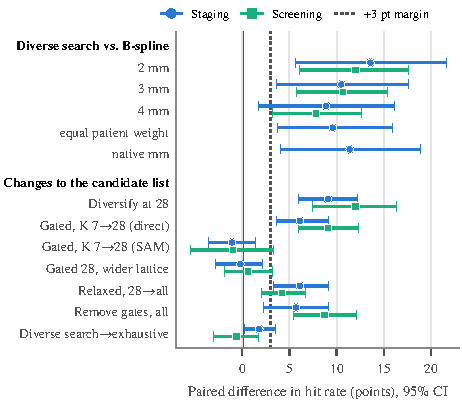
\includegraphics[width=\linewidth]{figures/paired_forest.pdf}
\caption{\textbf{Paired differences with 95\% patient-cluster intervals.} Top: \ours minus B-spline at three tolerances and in two robustness analyses (staging only). Bottom: changes to the candidate list at 3\,mm (Tab.~\ref{tab:contrasts}). The dashed line is the 3-point margin fixed before inference; an interval entirely to the right of zero is a significant gain.}
\label{fig:forest}
\end{figure}

\begin{figure*}[!t]
\centering
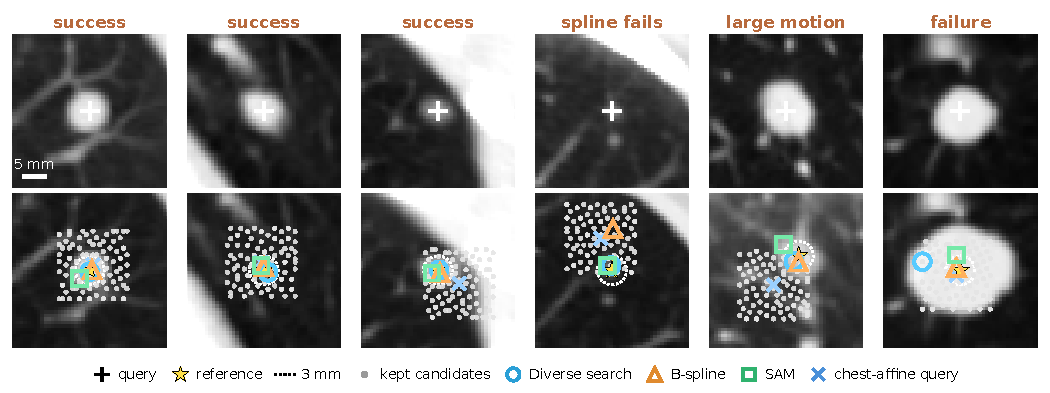
\includegraphics[width=\linewidth]{figures/qualitative.pdf}
\caption{Qualitative examples from the staging cohort. The columns are three successes, one spline failure, one large-motion case, and one failure of Diverse search. Top: current CT with the query ($+$). Bottom: earlier CT with the reference (star) and a 3 mm tolerance (dotted), the kept candidates (small dots), and the points selected by Diverse search (circle), the B-spline (triangle), and SAM (square). The cross is where the chest affine places the query.}
\label{fig:qualitative}

\end{figure*}

\subsection{Sensitivity to the query}
\label{sec:query}
Because the query is simulated by jittering the annotated mark, part of the gain could come from lesions whose query starts far away.
Figure~\ref{fig:bands} splits lesions by the distance between the query $p$ and the annotated current mark.
Among lesions whose query is within 1.5\,mm, \ours hits 238 of 322 staging lesions versus 205 for the spline ($+10.2$ points [2.1, 18.4]) and 178 versus 157 of 194 screening lesions ($+10.8$ [5.8, 16.0]).
This well-localized band contributes 33 of the 46 net staging gains and 21 of the 33 screening gains.
The smaller bands have wide intervals and are descriptive.

We also reran the screening cohort with the exact annotated mark as the query.
The spline improves from 211 to 239 hits, while \ours is essentially unchanged (244 to 243).
With a perfect query the screening advantage therefore shrinks from 33 to 4 hits, so a large part of it reflects robustness to an imprecise query (supplement, Tab.~S7).
We return to this in Sec.~\ref{sec:discussion}.

\begin{figure}[!t]
\centering
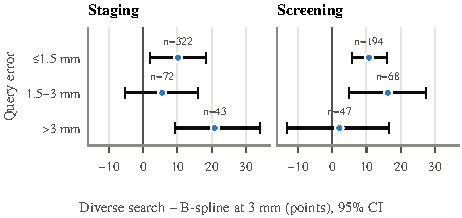
\includegraphics[width=\linewidth]{figures/query_bands.pdf}
\caption{\textbf{Gain by query error.} Paired 3\,mm difference between \ours and the B-spline within bands of query error (distance between $p$ and the annotated current mark), with 95\% patient-cluster intervals; $n$ is the number of lesions per band. Three unsupported staging queries are excluded here but counted in Tab.~\ref{tab:main}.}
\label{fig:bands}
\end{figure}

\subsection{Diversification makes better use of a fixed budget}
\label{sec:diversity}
At a budget of 28, the fit-ordered list spends several slots on the same neighborhood.
Enforcing 2.1\,mm separation, with the same order, grid and scorer, raises reach from 221 to 274 staging lesions and from 189 to 242 screening lesions, and raises hits from 205 to 245 ($+9.1$ points [6.0, 12.2]) and from 175 to 212 ($+12.0$ points [7.5, 16.4]) (Tab.~\ref{tab:contrasts}).
Figure~\ref{fig:attribution} applies Eq.~\ref{eq:decomp}.
Diversification makes 54 staging and 56 screening lesions newly reachable, and the scorer selects 45 and 41 of them, while choices on lesions reachable by both lists lose a net four hits in each cohort.
The gain is therefore a gain in coverage, not in selection.
The same holds with relaxed gates, where diversification at 28 adds 7.5 [4.7, 10.7] and 9.4 [5.3, 13.4] points.

\begin{figure}[!t]
\centering
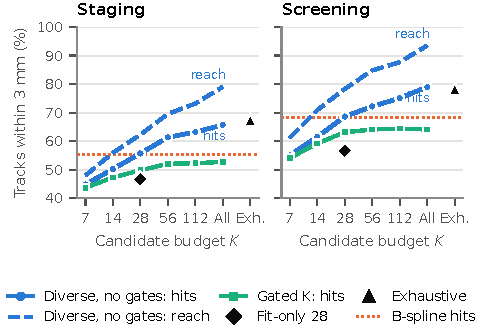
\includegraphics[width=\linewidth]{figures/budget_reach.pdf}
\caption{\textbf{Reach and hits versus candidate budget} at fixed wide extent and image support. Dashed: share of lesions with any candidate within 3\,mm (reach). Solid: share whose selected point is within 3\,mm (hits). At $K{=}28$ the diversified list (blue) beats the fit-only list (diamond) by 9.1 and 12.0 points; hard gates (green) limit the benefit of a larger budget. Exh.: all 4,851 positions.}
\label{fig:budget}
\end{figure}

\begin{table}[!t]
\centering
\footnotesize
\setlength{\tabcolsep}{2.2pt}
\begin{tabular}{@{}llccc@{}}
\toprule
& Change & Reach & Hits & $+$/$-$ \\
\midrule
\multirow{7}{*}{\rotatebox{90}{Staging}}
& Diversify at 28 & 221$\to$274 & 205$\to$245 & 51/11 \\
& Strict 7$\to$28, direct & 202$\to$241 & 192$\to$219 & 34/7 \\
& Strict 7$\to$28, SAM & 202$\to$241 & 144$\to$139 & 17/22 \\
& Wider lattice at 28 & 239$\to$241 & 220$\to$219 & 15/16 \\
& Relaxed 28$\to$all & 264$\to$300 & 237$\to$264 & 33/6 \\
& Remove gates, all & 300$\to$348 & 264$\to$289 & 30/5 \\
& Diverse$\to$exhaustive & 348$\to$351 & 289$\to$297 & 12/4 \\
\midrule
\multirow{7}{*}{\rotatebox{90}{Screening}}
& Diversify at 28 & 189$\to$242 & 175$\to$212 & 44/7 \\
& Strict 7$\to$28, direct & 185$\to$220 & 167$\to$195 & 28/0 \\
& Strict 7$\to$28, SAM & 185$\to$220 & 121$\to$118 & 23/26 \\
& Wider lattice at 28 & 220$\to$220 & 193$\to$195 & 9/7 \\
& Relaxed 28$\to$all & 235$\to$257 & 204$\to$217 & 14/1 \\
& Remove gates, all & 257$\to$289 & 217$\to$244 & 29/2 \\
& Diverse$\to$exhaustive & 289$\to$290 & 244$\to$242 & 6/8 \\
\bottomrule
\end{tabular}
\caption{Paired changes to the candidate list at 3\,mm on all 440 staging and 309 screening lesions. $+$/$-$ counts lesions that become hits / stop being hits. Differences in points with 95\% intervals are plotted in Fig.~\ref{fig:forest}.}
\label{tab:contrasts}
\end{table}


Figure~\ref{fig:budget} follows reach and hits as the budget grows.
The complete diversified list reaches 348 of the 351 lesions reachable on the full lattice in staging and 289 of 290 in screening, while scoring about one-thirteenth of the positions.
The coverage bound (Eq.~\ref{eq:coverage}) also predicts a cost: one kept point represents a cluster of nearby translations, which matters more at tight tolerances.
Indeed, exhaustive scoring adds 18 staging hits over \ours at 2\,mm but only five at 4\,mm.

\subsection{Additional reach pays off only with a capable scorer}
\label{sec:scorer}
Raising the strict cap from 7 to 28 increases direct hits from 192 to 219 on staging ($+6.1$ points [3.6, 9.1]) and from 167 to 195 on screening ($+9.1$ points [6.0, 12.3]), both above the prespecified margin.
Widening the lattice at fixed support and cap 28 does not help (intervals span zero), so the number and placement of kept candidates, not the lattice extent, drive the gain.
On the identical expanded lists, the direct scorer selects 33 of the 39 newly reachable staging lesions, whereas SAM selects only 10 and loses 15 hits on the 202 shared lesions (Fig.~\ref{fig:attribution}).
The cap effect favors the direct scorer over SAM by 7.3 points [4.4, 10.4] on staging and 10.0 [5.4, 14.8] on screening.
A larger candidate budget is useful only to a scorer that can exploit it.

\begin{figure}[!t]
\centering
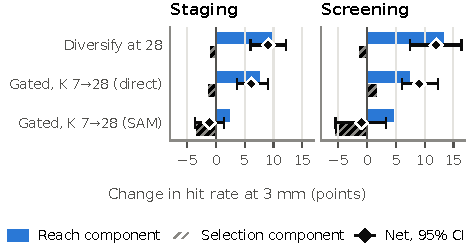
\includegraphics[width=\linewidth]{figures/reach_selection.pdf}
\caption{\textbf{Where additional hits come from} (Eq.~\ref{eq:decomp}), in points. Blue: reach term (hits on newly reachable lesions minus hits lost with reach). Hatched: selection term (change on lesions reachable by both lists). Black: net change with its 95\% interval. Diversification and a larger cap gain through reach with the direct scorer; SAM, given identical candidates, loses more on shared lesions than it gains.}
\label{fig:attribution}
\end{figure}

Hard gates also discard usable candidates.
With relaxed gates, replacing cap 28 by the complete list raises hits from 237 to 264 (staging) and from 204 to 217 (screening).
Removing the remaining gates adds 48 and 32 reachable lesions and 25 and 27 hits.
Since anatomical fit still enters Eq.~\ref{eq:direct}, this supports using fit as a soft preference rather than a hard filter.

\subsection{Compute}
\label{sec:latency}
On prepared staging crops, the median local time is 0.194\,s for \ours versus 3.617\,s for the spline (18.6$\times$), and 0.185 versus 3.866\,s on screening (20.9$\times$); p90 times are 0.458 versus 4.707\,s and 0.190 versus 4.693\,s.
Figure~\ref{fig:speed} places every fixed budget on one accuracy--latency plot.
The diversified 28-point list costs 22\,ms more than the fit-only list for 40 additional staging hits.
A cap of 112 gives 278 staging hits at 0.142\,s, saving a median 50\,ms [45, 53] per query relative to the complete list, an intermediate operating point.
With native scans, chest alignment dominates: one query per screening pair takes 29.36\,s for \ours versus 32.87\,s for the spline, and two queries sharing the alignment take 14.88 versus 19.38\,s per query.
The local speedup therefore matters most when the alignment is shared across many lesions.

\begin{figure}[!t]
\centering
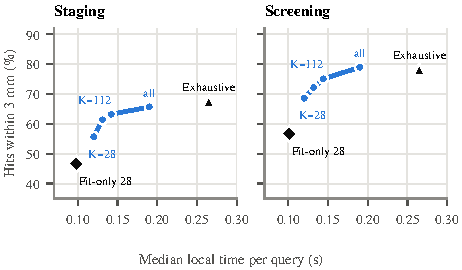
\includegraphics[width=\linewidth]{figures/accuracy_latency.pdf}
\caption{\textbf{Accuracy versus prepared-crop latency.} Diverse search at caps 28, 56, 112 and the complete list, the fit-only list and exhaustive scoring come from a three-repeat randomized replay on matched workloads of 24 staging and 32 screening queries; the spline point is from the matched prepared-crop comparison. Hit rates use the full cohorts.}
\label{fig:speed}
\end{figure}
